\documentclass[preprint]{sigplanconf}

% The following \documentclass options may be useful:
% preprint      Remove this option only once the paper is in final form.

\usepackage{amsmath}
\usepackage{graphicx}
\usepackage{hyperref}
\usepackage{url}

\newcommand{\ALGOL}{A\textsc{LGOL}}
\newcommand{\MATLAB}{\textsc{MATLAB}}
\newcommand{\Mathematica}{\textit{Mathematica}}
\newcommand{\code}[1]{\texttt{#1}}

\begin{document}

\special{papersize=8.5in,11in}
\setlength{\pdfpageheight}{\paperheight}
\setlength{\pdfpagewidth}{\paperwidth}

\conferenceinfo{ARRAY '14}{June 15, 2014, Edinburgh, UK}
\copyrightyear{2014} 
%\copyrightdata{978-1-nnnn-nnnn-n/yy/mm} 
%\doi{nnnnnnn.nnnnnnn}

% Uncomment one of the following two, if you are not going for the 
% traditional copyright transfer agreement.

%\exclusivelicense                % ACM gets exclusive license to publish, 
                                  % you retain copyright

\permissiontopublish             % ACM gets nonexclusive license to publish
                                  % (paid open-access papers, 
                                  % short abstracts)

\titlebanner{Array Operators Using Multiple Dispatch}    % These are ignored unless
\preprintfooter{Array Operators Using Multiple Dispatch} % 'preprint' option specified.

% \title{Array implementations in Julia}

%\title{Array Operators Using Multiple Dispatch}
%\subt
\title{ Array Operators Using Multiple Dispatch }
\subtitle{A design methodology for array implementations in dynamic languages}

\authorinfo{Jeff Bezanson \and Jiahao Chen \and Stefan Karpinski \and Viral Shah  \and Alan Edelman}
           {MIT Computer Science and Artificial Intelligence Laboratory}
  { bezanson@mit.edu, jiahao@mit.edu, stefan@karpinski.org, viral@mayin.org, edelman@mit.edu }

\maketitle

\begin{abstract}

Arrays are such a rich and fundamental data type that they tend to be built in to
a language, either in the compiler or in a large low-level library.
It would be better to define this functionality at the user level, providing more
flexibility for application domains not envisioned by the language designer.
Only a few languages, such as C++ and Haskell, provide the necessary power to define
$n$-dimensional arrays, but these systems rely on compile-time abstraction,
sacrificing some amount of flexibility.
In contrast, dynamic languages make it straightforward for the user to define any
behavior they might want, but at the possible expense of performance.

As part of the Julia language project, we have developed an approach that yields
a novel trade-off between flexibility and compile-time analysis. The core
abstraction we use is multiple dispatch.
We have come to believe that while multiple dispatch has not been especially popular
in most kinds of programming, technical computing is its killer application.
%This has been extensively studied
%as a general object-oriented programming technique, but we find it
%especially relevant to technical and array-based programming.
By expressing key functions such as array indexing using multi-method
signatures, a surprising range of behaviors can be obtained, in a way that is
both relatively easy to write and amenable to compiler analysis.
The compact factoring of concerns provided by these methods makes it easier
for user-defined types to behave consistently with types in the standard
library.

%pulls out abstractions that might not have been named before
%creates better integration of user-defined types
%flexible enough to change the behavior if you want
%creates more coherence

%Interest in recovering performance in these systems has spurred development of
%analysis frameworks. 

\end{abstract}

%\category{CR-number}{subcategory}{third-level}

\keywords
Julia, multiple dispatch, type inference, array indexing, static analysis,
dynamic dispatch

\section{Array libraries}

\begin{quotation}
``Unfortunately, it is very difficult for a designer to select in advance all
the abstractions which the users of his language might need. If a language is
to be used at all, it is likely to be used to solve problems which its
designer did not envision, and for which abstractions embedded in the language
are not sufficient.'' - Ref. \cite{Liskov:1974pb}
\end{quotation}

$n$-arrays (arrays of rank $n$, or simply `arrays') are an essential data
structure for technical computing, but are challenging to implement
efficiently \cite{Sattley:1960as,Sattley:1961as, Randell:1964a6}. There is a
long history of special-purpose compiler optimizations to make operations over
arrays efficient, such as loop fusion for array traversals and common
subexpression elimination for indexing operations \cite{Randell:1964a6,
Busam:1969oe}. Many language implementations therefore choose to build array
semantics into compilers.

However, only a few of the languages that support $n$-arrays have sufficient
power to express the semantics of $n$-arrays for general rank $n$ without
resorting to hard-coding array behavior into a compiler.
Notable examples include C++, with libraries like
\code{Blitz++} \cite{Veldhuizen:1998ab} or \code{Boost.MultiArray}
\cite{Garcia:2005ma}, and Haskell's Repa (Regular Parallel Arrays)
\cite{Keller:2010rs,Lippmeier:2011ep, Lippmeier:2012gp}. These libraries
leverage the static semantics of their host languages to
define $n$-arrays inductively as the outer product of a 1-array with an
$(n-1)$-array \cite{Bavestrelli:2000ct}.
A common pattern in such libraries is to handle dimensions one at a time,
recursively, so the compiler can understand each step.
Knowing array rank at compile time is valuable, since the amount of
storage needed for the dimension sizes is then known, and index
computations can be fully unrolled.

%This recursive peeling of rank thus
%defines general $n$-arrays. The dispatch semantics also allows for efficient
%implementations of certain operations; for example, \code{Repa} allows for in-
%memory transposition by dispatching on classes with different memory striding
%rules \cite{Keller:2010rs}. The use of compile-time features allows these
%libraries to eliminate runtime overhead for better performance.

\subsection{Static tradeoffs}

Array libraries built using compile-time abstraction have good performance,
but also some limitations.
First, features like C++ templates are not available at run time, so these
libraries do not support $n$-arrays where $n$ is known only at run time.
Second, code using these features is
notoriously difficult to read and write; it is effectively written in a
separate sub-language.
Third, the recursive strategy for defining $n$-arrays
naturally favors only certain indexing behaviors. For example,
\code{Repa}'s reductions like \code{sum} are only defined naturally over the
last index \cite{Keller:2010rs}; reducing over a different index requires
a permutation.
However, it is worth noting that Haskell's type system encourages
elegant factoring of abstractions. While the syntax may be unfamiliar,
we feel \code{Repa} ought to hold much interest for the technical computing
community.
%permutation operations and are not guaranteed to produce an optimal memory
%traversal pattern. The overhead incurred by general indexing operations can be
%avoided only by implementing many special cases that ensure maximal
%exploitation of loop unrolling optimizations and other similar static analyses
%\cite{Garcia:2005ma, Lippmeier:2011ep}, which engenders much repetition in the
%codebase \cite{Lippmeier:2012gp}.

Some applications call for semantics that are not amenable
to static analysis. Certain applications require arrays whose ranks are known
only at run time, and thus the data structures in these programs cannot be
guaranteed to fit in a constant amount of memory. Some programs may
wish to dynamically dispatch on the rank of an array, a need which a
library must anticipate by providing appropriate virtual methods.

%different semantics for arrays of different ranks. Some technical computing
%applications, for example, wish to treat vectors (1-arrays) differently from
%matrices (2-arrays), supporting computations such as the singular value
%decomposition for the latter but not the former. In such contexts, column
%vectors are no longer equivalent to $N\times1$ matrices or 2-arrays with a
%trailing singleton dimension, and programs that conflate them violate the
%Liskov substitution principle \cite{Liskov:1987da}, in ways are are analogous
%to the canonical circle-ellipse problem \cite{Halbert:1987ut}.

\subsection{Dynamic language approaches}

Applications requiring run time flexibility are better expressed in
dynamic languages such as \Mathematica, \MATLAB, R, and Python/NumPy, where
all operations are dynamically dispatched (at least semantically, if not
in actual implementation). Such flexibility,
however, has traditionally come at the price of slower execution.
To improve performance, dynamic languages typically resort to static analysis
at some level.
One strategy is to implement arrays in an external library
written in a static language.
The Python NumPy package is a prominent example, implementing array operations
as well as its own type system and internal abstraction mechanisms within
a large C code base. As a result, NumPy \code{ndarray}s are
superficially Python objects, but implementation-wise are disjoint from the
rest of the Python object system, since little of Python's native object
semantics is used to define their behavior.

Another approach is to implement static analyses
\textit{de novo} for dynamic languages. However, the flexibility
of these languages' programs limits the extent of analysis that is
realistically possible. For example, \MATLAB's array
semantics allow an array to be enlarged automatically whenever a write occurs
to an out-of-bounds index, and also for certain operations to
automatically promote the element type of an array from real to complex
numbers. This poses implementation challenges for static \MATLAB{} compilers
like \code{FALCON}, which have to implement a complete type system with
multiple compiler passes and interprocedural flow analyses to check
for such drastic changes to arrays \cite{Rose:1999tt,
Li:2013mf}. Additionally, type checking is essential to disambiguate
\MATLAB{} expressions like \code{A*B}, which, depending on the dimensions of
\code{A} and \code{B}, could represent a scaling, inner product, outer
product, matrix-matrix multiplication, or matrix-vector multiplication
\cite{Rose:1999tt}. Similar work has been done for other dynamic languages,
as in Hack, a PHP implementation with a full static type system
\cite{Verlaguet:2014hn}.

%TODO other languages: APL, ZPL, Lisp?

The conflicting requirements of performance and flexibility pose a dilemma for
language designers and implementers. Most current languages choose either to
support only programs that are amenable to static analysis for the sake of
performance, like C++ and Haskell, or choose to support more general
classes of programs, like \MATLAB, \Mathematica, and Python/NumPy. While
dynamic languages nominally give up static analysis in the process, many
implementations of these languages still resort to static analysis in
practice, either by hard-coding array semantics in a post-hoc compiler, or by
implementing arrays in an external library written in a static language.

%A key problem with dynamic languages is how to provide more declarative
%information to a compiler. Users expect to be able to program any
%run-time behavior and have it just work. In theory, a compiler could
%partially evaluate programs based on whatever static information it can
%find (e.g. integer constants), but it is unlikely that this would reliably
%provide performance where it is needed.

%The user should not have to learn two different sets of semantic behavior. In Julia, that's the compiler's job. It does mean that the it's not as fast as a static language.

%TODO need some words to connect to Figure~\ref{fig:langdesign}

\begin{figure}
  \centering
  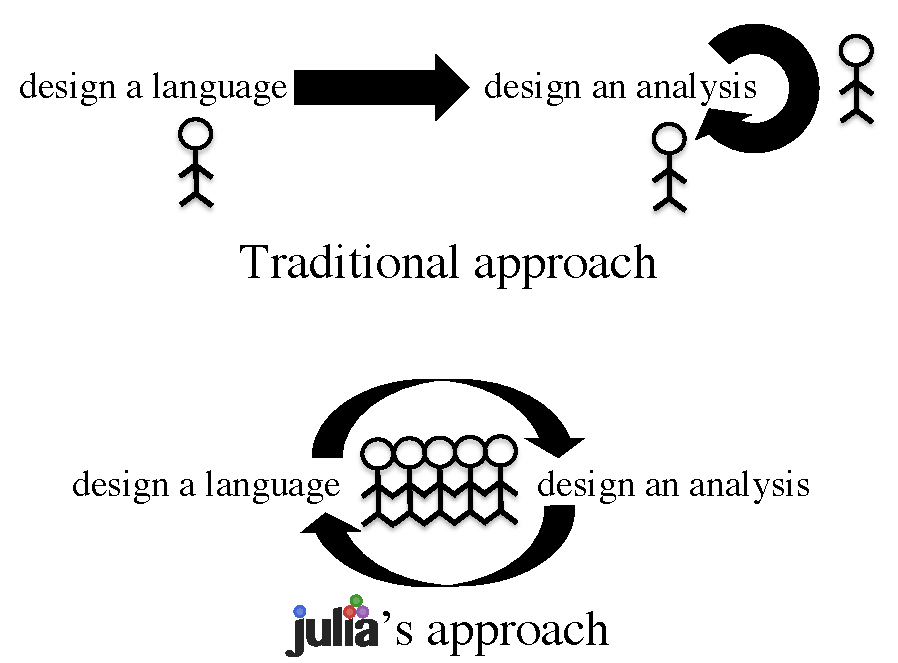
\includegraphics[width=\columnwidth]{fig-langdesign}
  \caption{\label{fig:langdesign}
Most dynamic languages are designed without consideration for program analysis,
leaving this to other, future compiler writers and researchers who step in if
the language becomes popular enough to warrant it.
Julia is designed with analysis in mind, with a single community responsible for both
language design and performant implementation. This approach is natural for
statically-typed languages, but dynamic languages need static analysis too.}
\end{figure}

\section{Julia arrays}

Julia is dynamically typed and is based on dynamic multiple dispatch.
However, the language (and its standard library) have been designed to
take advantage of the possibility of static analysis
(Figure~\ref{fig:langdesign}), especially
dataflow type inference. In this section we will describe some features
of the array implementation that arise from this design decision.

Arrays are implemented in Julia\cite{Bezanson:2012jf} as the \code{Array}
data type, which is parameterized by an element type and a rank (an integer).
For purposes of this paper, an \code{Array} can be considered a tuple of
a contiguous memory region and a shape (a tuple of integers giving the size
of the array in each dimension). This simple representation is already
enough to require nontrivial design decisions.

%% Multiple dispatch makes it possible for \code{Array}s to have implementations
%% that afford both generality and efficiency. The most general
%% \code{Array\{Any\}} is an array of pointers to heap-allocated values. However,
%% \code{Array}s of native machine types like double precision floating point
%% numbers (\code{Float64}s) or integers of native machine size (\code{Int}s) can
%% be implemented to be C/Fortran- compatible. Interestingly,
%% \code{Array\{Nothing\}} can be implemented with zero storage space at runtime,
%% since it consists of elements of an immutable type with zero fields, which is
%% possible because only a single instance of any such type can exist, and hence
%% need not actually be stored. This allows for some clever tricks like
%% implementing \code{Set\{T\}} using a \code{Dict\{T,Nothing\}} to avoid paying
%% any cost for the value array in the \code{Dict}.

%TODO identify subthemes in this giant block
%The implementation of Julia \code{Array}s differs significantly from other
%languages in several important respects. First, automatic type inference is
%not used merely as a compiler optimization technique, like in static compilers
%for dynamic languages, but instead is a crucial language feature that, in
%conjunction with multiple dispatch, are necessary for implement language
%semantics. Second, Julia by virtue of being a dynamic language provides the
%static analyses enabled by type inference and multiple dispatch at runtime. In
%contrast, C++ templates are static semantics that are
%unavailable at runtime, and the semantics of templates are for the purposes of
%runtime programs effectively a separate language. The single all- runtime
%model of Julia is much easier to use and imposes fewer restrictions on the
%kind of Julia code that can be written.

%You can implement a bigger class of
%rules in Julia rather than having to special case on the number of dimensions
%or be forced to rely on recursive definitions onto subarrays.

%For example in
%Julia you can do \code{A[I...]} where \code{I} is a heterogeneous array, and
%all the same definitions are still applicable, but you might take a bit of
%performance drop.

%Third, Julia aggressive employs specialization on argument
%types by default, generating a large variety of specialized methods for each
%generic function, in contrast with the default of one compilation per function
%declaration in most other languages. This is possible thanks to the static
%analyses enabled by type inference and multiple dispatch. C++ can do this with
%templates, but generating an entire family of related methods must be
%requested explicitly using templates. Furthermore, having all the semantics
%enabled by static analysis at runtime allows for composition for code that
%results in efficient specialized methods by the compiler. For example, Julia
%code implementing the algebra of the quaternion field can be composed
%transparently with other Julia code implementing Gaussian elimination by the
%compiler. One can be inlined into the other and woven into a specialized
%method for Gaussian elimination on quaternionic matrices. Contrast this with
%the conventional wisdom that user-defined types are slow in languages like
%\MATLAB{} and

%even C++; user-defined classes are reference types rather than
%value types, and methods have to be declared \code{virtual} to enable dynamic
%dispatch as opposed to the default static dispatch mechanism. In Julia,
%everything in principle has to happen dynamically but then the focus is on
%analyzing it statically.

%Fourth, array functions in Julia have access to the
%entire argument list, allowing for conceptual models and APIs that are not
%restricted to strict left-to-right or right-to-left index traversal that would
%be necessary by recursive peeling. Fifth, specialization of methods can be
%implemented with multiple dispatch, which is a powerful alternative to the
%single dispatch mechanism of Haskell based on function classes and pattern
%matching.

%In the cases where static analysis can happen, Julia can perform as fast as
%languages where array semantics is predicated on static analysis, but multiple
%dispatch allows Julia to be more flexible than just this. Julia also allows
%for generic fall-back methods that are slower because of a lack of static
%analysis, but nonetheless can be dispatched upon. The flexibility that is
%allowed by this approach is a nonobvious application of multiple
%dispatch.

\subsection{Array indexing rules}

Rules must be defined for how various operators act
on array dimensions. Here we will focus on indexing, since selecting parts of
arrays has particularly rich behavior with respect to dimensionality. For
example, if a single row or column of a matrix is selected, does the result
have one or two dimensions? Array implementations prefer to invoke general
rules to answer such questions. Such a rule might say ``dimensions indexed
with scalars are dropped'', or ``trailing dimensions of size one are
dropped'', or ``the rank of the result is the sum of the ranks of the
indexes'' (as in APL).

The recursive approach favored in static languages tends to force this
design decision. For example, in C++ a 3-dimensional indexing
expression might be written as \code{A[i][j][k]}. Here there are three
applications of \code{operator[]}, each of which will decide whether to
drop a dimension based on the type of a single index. The second rule
described above, and others like it, cannot be implemented in such a
scheme.

Our dispatch mechanism permits a novel approach that encompasses more
rules, and does not require array rank to be known statically but
benefits when it is.
This solution is still a compromise among the factors outlined in
the introduction, but it is a new compromise that we find compelling.

%Here we consider the indexing rules. How to compute shapes of subarrays. How
%to deal with singleton dimensions is but a special case even though
%superficially the rules mention them explicitly.

%In Julia, such indexing rules are defined in exactly one place and can be
%changed later if so desired.

\subsection{The need for flexibility}

Our goal here is a bit unusual: we are not concerned with which rules might
work best, but merely with how they can be specified, so that domain experts
can experiment.

In fact different domains want different things. In image processing for
example, each dimension might be quite different, e.g. time vs. space vs. color,
so you don't want to drop or rearrange dimensions too often. In linear algebra
on the other hand, one might want a row or column of a matrix to become a vector
by dropping a dimension.

In practice we may have to reach a consensus on what rules to use, but this
should not be forced by technical limitations.

%% (jeff says) TODO: these look like good examples but I don't know enough about
%% them to flesh this out.
%In Julia, these are not enforced a priori. Sometimes the
%distinctions between the various indexing rules are semantically meaningful
%and that's when this flexibility becomes particularly valuable. For example
%Tim Holy's image 4-arrays. Quantum mechanics when you average out multiple
%indistinguishable particles. $n$-point correlations functions where which $k$
%indices you average out defines any number of lower-point $n-k$ point
%correlation functions.

%% Instead of the compiler analyzing indexing expressions and determining an
%% answer using hard-coded logic, we would rather implement the behavior in
%% libraries, so that different kinds of arrays may be defined, or so that rules
%% of similar complexity may be defined for other kinds of objects. But these
%% kinds of rules are unusually difficult to implement in libraries. If a library
%% writes out its indexing logic using imperative code, the host language
%% compiler is not likely to be able to analyze it.

%Why is it important to be able to express this in a library? No hidden
%theories, some sort of consistency. Another reason is heuristic, don't really
%know what people want in the future. Put in what people know now, hope that
%the next generation will still have the flexibility to modify it to their
%needs.

\subsection{Multiple dispatch}

Multiple dispatch (also known as generic functions, or multi-methods) is an
object-oriented paradigm where methods are defined on combinations of data
types (classes), instead of encapsulating methods inside classes
(Figure~\ref{fig:dispatch}). Methods are
grouped into generic functions. A generic function can be applied to several
arguments, and the method with the most specific signature matching the
arguments is invoked.

\begin{figure}
  \centering
  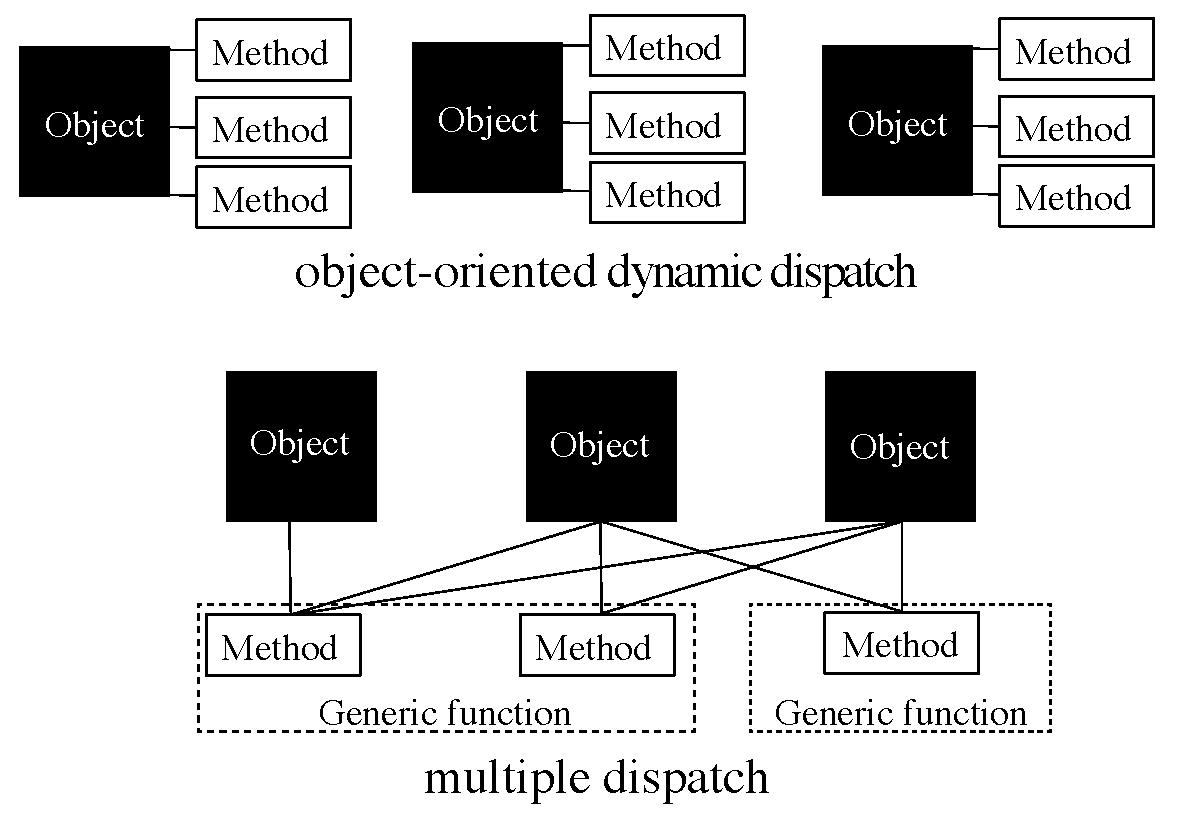
\includegraphics[width=\columnwidth]{fig-md-oo}
  \caption{\label{fig:dispatch}Class-based method dispatch vs. multiple dispatch.}
\end{figure}

One can invent examples where multiple dispatch is useful in classic OO domains
such as GUI programming. A method for drawing a label onto a button might
look like this in Julia syntax:

\begin{verbatim}
function draw(target::Button, obj::Label)
    ...
end
\end{verbatim}

In a numerical setting, binary operators are ubiquitous and we can easily imagine
needing to define special behavior for some combination of two arguments:

\begin{verbatim}
+(x::Real, z::Complex) = complex(x+real(z), imag(z))
\end{verbatim}

But how much more is there? Would we ever need to define a method on
\emph{three} different types at once? Indeed, most language designers and
programmers seem to have concluded that multiple dispatch might be nice, but is
not essential, and the feature is not often used \cite{Muschevici:2008}.
%TODO: cite statistic from study of multiple dispatch showing it is lightly used
Perhaps the few cases that seem to need it can be handled using tricks like
Python's \code{\_\_add\_\_} and \code{\_\_radd\_\_} methods.

However, multiple dispatch looks quite different in the context of technical
computing. To a large extent, technical computing is characterized
by the prevalence of highly polymorphic, multi-argument operators. In many
cases, these functions are even more complex than the 2-argument
examples above might indicate. To handle these, we have added a few
features that are not always found in multiple dispatch implementations.

For this paper, perhaps the most important of these is support for
variadic methods. Combining multiple dispatch and variadic methods
seems straightforward
enough, and yet it permits surprisingly powerful definitions. For example,
consider a variadic \code{sum} function that adds up its arguments. We could
write the following two methods for it (note that in Julia, \code{Real} is
the abstract supertype of all real number types, and \code{Integer} is the
abstract supertype of all integer types):

\begin{verbatim}
sum(xs::Integer...)
sum(xs::Real...)
\end{verbatim}

The syntax \code{...} allows an argument slot to match any number of trailing
arguments (currently, Julia only allows this at the end of a method signature).
In the first case, all arguments are integers and so we can use a naive
summation algorithm. In the second case, we know that at least one argument
is not an integer, so we might want to use some form of compensated
summation instead. Notice that these modest method signatures
capture a subtle property (at least one argument is non-integer)
\emph{declaratively}: there is no need to explicitly loop over the arguments
to examine their types. The signatures also provide useful type information:
at the very least, a compiler could know that all argument values inside
the first method are of type \code{Integer}. Yet the type annotations
are not redundant: they are necessary to specify the desired behavior. There
is also no loss of flexibility: \code{sum} can be called with any combination
of number types, as users of dynamic technical computing languages would expect.

While the author of these definitions does not write a loop to examine
argument types, such a loop of course still must take place somewhere inside
the dispatch system. Such a complex dispatch system is naturally at risk of
performing badly. However, Julia pervasively applies dataflow type
inference, so that argument types are often known in advance, in turn
allowing method lookup to be done at compile time. Technically this is
just an optimization, but in practice it has a profound impact on how code
is written.

\subsection{\code{index\_shape}}

Multiple dispatch appears at first to be about operator overloading:
defining the behavior of functions on new, user-defined types.
But the fact that the compiler ``knows'' the types of function arguments leads
to a surprising, different application: performing elaborate, mostly-static,
transformations of argument tuples.

Determining the result shape of an indexing operation is just such a
transformation. In Julia's standard library, we have a function
\code{index\_shape} that accepts index arguments (which, for present
purposes, may be scalars or arrays of any rank), and returns the
shape (a tuple of integers) of the result. The length of the shape
determines the rank of the result array. Many different behaviors
are possible, but currently we use the rule that trailing dimensions
indexed with scalars are dropped\footnote{This rule is the subject of
some debate in the Julia community. Fortunately it is easy to change,
as we will see.}.
For example:

\begin{verbatim}
A[1:m, 1:n, 2]     # rank 2
A[1:m, 2, 1:n]     # rank 3
A[1:m, 2, 1:n, 1]  # rank 3
\end{verbatim}

The following two method definitions express this behavior:

{\small
\begin{verbatim}
# drop trailing dimensions indexed with scalars
index_shape(i::Real...) = ()
index_shape(i, I...)    = tuple(length(i),
                                index_shape(I...)...)
\end{verbatim}
}

(The syntax \code{...} within an expression, on the right-hand side of
a definition, performs ``argument splicing'': the elements of a container
are spread into multiple arguments to the called function. Formal
arguments that lack a \code{::} type specializer match any value.)
The first definition traps and collapses runs of \code{Real} arguments of
any length. The second definition ensures that the first definition only
applies to the tail of an argument tuple, by keeping indexes as long as
some non-scalar arguments remain.

Since all indexing functions call this function, changing these two lines is
sufficient to change how indexing works. For example, another rule one might
want is to drop \emph{all} dimensions indexed with scalars:

{\small
\begin{verbatim}
# drop dimensions indexed with scalars
index_shape()              = ()
index_shape(i::Real, I...) = index_shape(I...)
index_shape(i, I...)       = tuple(length(i),
                                   index_shape(I...)...)
\end{verbatim}
}

Or we could immitate APL's behavior, where the rank of the result is the sum
of the ranks of the indexes, as follows:

{\small
\begin{verbatim}
# rank summing (APL)
index_shape()        = ()
index_shape(i, I...) = tuple(size(i)...,
                             index_shape(I...)...)
\end{verbatim}
}

Here \code{size} (as opposed to \code{length}) gives the shape tuple of an array,
so we are just concatenating shapes.


\subsection{Why it works}

Julia's multi-methods were designed with the idea that dataflow type inference
\cite{Cousot:1977, kaplanullman}
would be applied to almost all concrete instances of methods, based on
run-time argument types or compile-time estimated argument types. Without this
piece of infrastructure, definitions like those above might be no more
than a perversely slow way to implement the functionality. But with it, the
definitions have the effect of ``forcing'' the analysis to deduce accurate
types. In effect, such definitions are designed to exploit the dataflow
operation of matching inferred argument types against method signatures,
thereby destructuring and recurring through argument tuples at compile time.

Tuple types (or product types) are crucial to this analysis. Since the type
of each element of a tuple is tracked, it is possible to deduce that
the type of \code{f(x...)}, where \code{x} has tuple type \code{(A,B)}, is
equal to the type of \code{f} applied to arguments of types \code{A} and
\code{B}. Variadic methods introduce unbounded tuple types, written as
\code{(T...)}. Unbounded tuple types form a lattice of infinite height,
since new subtypes can always be constructed in the sequence
\code{(T...)}, \code{(T,T...)}, \code{(T,T,T...)}, etc. This adds
significant complexity to our lattice operators.

\subsection{Implications}

In a language with de-coupled design and analysis passes, a function like
\code{index\_shape} would be implemented inside the run-time system
(possibly scattered among many functions), and separately embodied in
a hand-written transfer function inside the compiler. Our design shows
that such arrangements can be replaced by a combination of high-level code and
a generic analysis (the Telescoping Languages project \cite{telescoping}
also recognized the value of incorporating analyzed library code into a
compiler).

From the programmer's perspective, Julia's multi-methods are convenient
because they provide run-time and compile-time abstraction in a single
mechanism. Having learned Julia's ``object'' system, one has also learned
its ``template'' system, without different syntax or reasoning about
binding time. Semantically, methods always dispatch on run-time
types, so the same definitions are applicable whether types are known
statically or not. Initially, a programmer's intent may be for all types
to be known statically. But if needs change and one day array rank needs
to be a run time property, the same definitions still work (with the only
difference being that the compiler will generate a dynamic dispatch or
two where there were none before). It is also possible to use popular
dynamic constructs such as \code{A[I...]} where \code{I} is a heterogeneous
array of indexes.
%Therefore users are free to reason about
%programs operationally, while gaining richer compile-time information
%as their method definitions grow more sophisticated.

One price of this flexibility is that not all such definitions are well-founded:
it is possible to write methods that yield tuples of indeterminate length.
The compiler must recognize this condition and apply widening operators
\cite{Cousot:1977, widening}. In these cases, the deduced types are
still correct but imprecise, and in a way that depends on somewhat arbitrary
choices of widening operators (for example, such a type might look
like \code{(Int...)} or \code{(Int,Int...)}).


\subsection{Symbolic programming}

Similarities to symbolic pattern-matching (as typically found in
computer algebra systems) are readily apparent. These systems effectively
allow dispatch on the full structure of values, and so are in some sense
even more powerful than our generic functions. However, they lack a clear
separation between the type and value domains, leading to performance
opacity: it is not clear what the system will be able to optimize
effectively and what it won't.

This could potentially be addressed by
designating some class of patterns as the ``types'' that the compiler
will analyze. However, more traditional type systems could be seen as
doing this already, while also gaining data abstraction in the bargain.

%TODO: point out how this combines the ``object part'' and the ``array part''
%into a coherent whole.
%This is really a statement about implementing array semantics in language X
%using language X itself, and in particular using intrinsic features for handling
%objects to also handle arrays.

%This approach does not depend on any heuristics. Each call to
%\texttt{index\_shape} simply requires one recursive invocation of type
%inference. This process reaches the base case \texttt{()} for these
%definitions, since each recursive call handles a shorter argument list (for
%less-well-behaved definitions, we might end up invoking a widening operator
%instead).

%\begin{verbatim}
%diverge() = randbool() ? () : tuple(1, diverge()...)
%\end{verbatim}

%This is an example of indexing behavior that is not amenable to useful static
%analysis, since each branch of \code{diverge()} has different types.

%TODO say something about how types of tuples in Julia are defined.

%Such code would throw a type error in languages requiring static
%checking such as Haskell. But in Julia, this is still allowed just that
%the compiler may not have useful information from static analysis and so may
%not run as fast. In Repa, the top priority is to appease the type system of
%Haskell, with performance and user interface secondary. We think it should be
%the other way round.

\section{Other applications}

Julia users have found many compelling applications of our multi-method
paradigm.

\subsection{Array views}

In certain instances of array indexing, it is
possible to keep the data in place and return just a view (pointer) to the
data instead of copying it. This functionality is implemented in a Julia
package called \code{ArrayViews.jl}\cite{Lin:2014av}. A crucial property
of an array view is its \emph{contiguous rank}: the number of leading
dimensions for which the strides equal the cumulative product of the shape.
When a view is constructed of another view, the type of view constructed
depends on the indexes used and the contiguous rank of the argument. In
favorable cases, a more efficient \code{ContiguousView} is returned.

This determination is made by a definition similar to the following:

{\small
\begin{verbatim}
function view(a::DenseArray, I::Subs...)
    shp = vshape(a, I...)
    make_view(a, restrict_crank(contrank(a, I...), shp),
              shp, I...)
end
\end{verbatim}
}

\code{contrank} essentially counts the number of leading ``colons'' in the
indexing expression. \code{make\_view} selects (via dispatch) what kind of
view to return based on the result type of \code{restrict\_crank}, which is
set up to return the smaller of its two argument shapes.
This is an excellent example of a library that needs to define behaviors
actually exceeding the complexity of what is provided in the standard library.

\subsection{Distributed arrays}

Other classes of array indexing rules are needed in distributed array
implementations. The Star-P system \cite{parry, Choy05parallelmatlab}
let users ``tag'' dimensions as potentially distributed using the notation
\code{*p}, which constructed a special type of object tracked by the system.
Indexing leads to questions of whether to take the first instance of \code{*p}
as the distributed dimension, the last instance, or perhaps just the last dimension.

Such distribution rules could be implemented and experimented with readily
using an approach similar to that used for \code{index\_shape}.

%Though not yet tested, an intriguing thought is that distributed array distribution
%rules can make use of the same approach as general array semantics.
%An interesting example is the  *p syntax used in Star-P. \cite{}
%In this syntax, array dimensions were listed as parallel with the *p notation.
%Julia multiple dispatch syntax provides the flexibility to explore the myriad of choices readily and flexibly.


\subsection{Unit quantities}

A package providing unitful computations (\code{SIUnits.jl}\cite{Fischer:2014si})
makes use of the same kinds of
tradeoffs as array semantics. Unitful computations are another case
where the relevent metadata (exponents on units) can be
known at compile time in many cases, but not always. The
\code{SIUnits} library is free to express the general case, and have the
overhead of tagging and dispatching removed where possible.



\section{Conclusion}

Programming languages must compromise between the ability to perform
static analyses and allowing maximal flexbility in user programs. Performance-
critical language features like arrays benefit greatly from static analyses,
and so even dynamic languages that initially lack static analyses eventually
want them one way or another.

We speculate that, historically, computer scientists developing multiple dispatch
were not thinking about technical computing, and those who cared about
technical computing were not interested in the obscurer corners of object oriented
programming. However we believe that the combination of dataflow type inference,
sophisticated method signatures, and the need for high-productivity technical
environments is explosive. In this context multi-methods, while still
recognizable as such, can do work that departs significantly from familiar
uses of operator overloading. By itself, this mechanism does not address
many of the concerns of array programming, such as memory access order
and parallelism. However, we feel it provides a useful increment of power
to dynamic language users who would like to begin to tackle these and other
related problems.

%% multiple
%% dispatch is not merely an optimization hack, but instead can be used to design
%% a programming language where they become core semantic features. The
%% implementation of these features in Julia is a remarkably efficient way to
%% allow code to be specialized to leverage static analyses for performance, yet
%% at the same time allows for other code written for maximal flexibility even in
%% the absence of detailed type information. Static analyzability becomes no
%% longer a property of an entire language, but instead an optional property of
%% specific programs in a particular language. Julia is therefore sufficiently
%% expressive to write complex, generic, dynamic multidimensional behaviors, and
%% more generally allows us to address the performance---flexibility compromise
%% in Julia with greater Pareto optimality than other existing solutions.

%\appendix
%\section{Appendix Title}
%
%This is the text of the appendix, if you need one.

\acks

The authors gratefully acknowledge the enthusiastic participation of the Julia
developer community in many stimulating discussions, in particular Dahua Lin and
Keno Fischer for the \code{ArrayViews.jl}\cite{Lin:2014av} and
\code{SIUnits.jl}\cite{Fischer:2014si} packages, respectively. Funding for this
work was supported by the MIT Deshpande Center, an Intel Science and
Technology award, a grant from VMWare, Citibank, a Horizontal Software
Fellowship in Compuational Engineering, and NSF DMS-1035400.

% We recommend abbrvnat bibliography style.

\bibliography{refs}{}
\bibliographystyle{abbrvnat}

% The bibliography should be embedded for final submission.

%\begin{thebibliography}{}
%\softraggedright

%\bibitem[Smith et~al.(2009)Smith, Jones]{smith02}
%P. Q. Smith, and X. Y. Jones. ...reference text...

%\end{thebibliography}

\end{document}
